\phantomsection
\chapter{Results}
\label{chap:eval_results}

\noindent Two kinds of results have been obtained. First results have been obtained by extracting a test set from the KDEF database, and test it against other subjects from the database. Feature extraction is done by LBP, followed by classification using SVM. The second set of results is obtained with the Kinect in real-time conditions, while the entire KDEF database is used for training. The Kinect gets video sequences of a subject in front of it, his or her face being extracted from these sequences using Viola-Jones algorithm. Then the same feature extraction and classification process is applied to these images.
\newline

\phantomsection
\section{First result set}

\vspace{\baselineskip}
\noindent To train the model, 128 face images from the KDEF database have been used for each emotion, plus neutral state. In total, $ 128\times7 = 896 $ face images have been used as train data. To test the system, 12 face images from the KDEF database have been used for each emotion, plus neutral state. In total, $ 12\times7 = 84 $ faces images have been used as test data. For each of these 84 images, face detection was performed first, then the uniform LBP operator extract its features, and then classification is performed using SVM.
\newline

\noindent The model has been trained with different kernels and different parameters. The outcome of these different processes are summed up in Table~\ref{table_results_kernels}. \textbf{\color{red} BLA BLA quel est le meilleur kernel, quelles différences et tout et tout}
\newline

\begin{table}[h]
\begin{center}
   \caption{\label{table_results_kernels} Results with different kernels and different parameters}
\begin{tabular}{|c|c|c|c|c|c|c|c|c|}
  \hline
    & Linear & \textbf{Poly1} & Poly2 & RBF1 & RBF2 & Sigmoid1 & Sigmoid2 \\
  \hline
  neutral & 66.00\% & \textbf{83.33\%} & 83.33\% & 83.33\% & 66.67\% & 8.33\% & 66.67\% \\
  afraid & 58.33\% & \textbf{83.33\%} & 75.00\% & 66.67\% & 66.67\% & 66.67\% & 58.33\% \\
  angry & 41.67\% & \textbf{41.67\%} & 33.33\% & 50.00\% & 41.67\% & 16.67\% & 41.67\% \\
  disgusted & 58.33\% & \textbf{75.00\%} & 75.00\% & 50.00\% & 50.00\% & 16.67\% & 58.33\% \\
  happy & 100.00\% & \textbf{100.00\%} & 91.67\% & 91.67\% & 100.00\% & 66.67\% & 100.00\% \\
  sad & 8.33\% & \textbf{8.33\%} & 0.00\% & 8.33\% & 8.33\% & 8.33\% & 8.33\% \\
  surprised & 66.67\% & \textbf{75.00\%} & 75.00\% & 66.67\% & 66.67\% & 25.00\% & 66.67\% \\
  \textbf{overall} & \textbf{57.14\%} & \textbf{66.67\%} & \textbf{61.90\%} & \textbf{59.52\%} & \textbf{57.14\%} & \textbf{29,76\%} & \textbf{57.14\%} \\
  \hline
\end{tabular}
<<<<<<< HEAD
=======
\end{center} 
>>>>>>> f3a1177041b834dbad80cc320be587f28fef16e6
\end{table}

\noindent \textit{Poly1} stands for Polynomial and has degree parameter: $ D = 2 $
\newline
\noindent \textit{Poly2} stands for Polynomial and has degree parameter: $ D = 3 $
\newline
\noindent \textit{RBF1} has cache and $\gamma$ parameters: $ C = 128 $ and $ \gamma = 0.0078125 $
\newline
\noindent \textit{RBF2} has cache and $\gamma$ parameters: $ C = 8192 $ and $ \gamma = 0.00048828125 $ 
\newline
\noindent \textit{Sigmoid1} has cache and $\gamma$ parameters: $ C = 128 $ and $ \gamma = 0.0078125 $
\newline
\noindent \textit{Sigmoid2} has cache and $\gamma$ parameters: $ C = 8192 $ and $ \gamma = 0.00048828125 $
\newline

<<<<<<< HEAD
\noindent A model has also been trained with same kernels and parameters but using cross-validation (as explained in Chapter \ref{chap:implementation_svm}). Results obtained with a model using cross-validation are compared to those with a model trained normally, this comparison being shown in  Table~\ref{table_results_crossvalidation}. All results are inferior or equal to those without cross-validation, except for linear and sigmoid kernels, with the latter tuned with the second set of parameters. 
=======
\noindent As said in Chapter \ref{chap:implementation_svm}, the parameters for the RBF and sigmoid kernel are find by the \textit{gridsearch} script of the SVM library. For the polynomial kernel, as said in Chapter \ref{chap:implementation_svm}, the $D$ parameter has to be chosen. By default, the $D$ parameter has the value 3. \textit{Poly2} has this value as parameter. For \textit{Poly1}, the $D$ parameter is $2$. It has been chosen because if the dimension is superior to $3$ then there is the problem of \textit{over-fitting}. It means that the model has good results but it is of use for this kind of data only. It has become to precise. And the gain in accuracy of adding one dimension does not worth it.
\newline

\noindent The same data has been trained with the same kernels and parameters but using cross-validation (as explained in Chapter \ref{chap:implementation_svm}). All results are inferior or equal to those without cross-validation, except for the sigmoid kernel with cache and $\gamma$ parameters equals to $ C = 8192 $ and $ \gamma = 0.00048828125 $. The table~\ref{table_results_crossvalidation} represents both results with and without cross validation.
>>>>>>> f3a1177041b834dbad80cc320be587f28fef16e6
\newline

\begin{table}[h]
\begin{center}
   \caption{\label{table_results_crossvalidation} Results with and without cross validation}
\begin{tabular}{|c|c|c|c|c|c|c|c|c|}
  \hline
    & with cross validation & without cross validation \\
  \hline
  Linear & 57.14\% & 57.14\% \\
  Poly1 & 55.95\% & 66.67\% \\
  Poly2 & 47.62\% & 61.90\% \\
  RBF1 & 52.52\% & 59.52\% \\
  RBF2 & 55.95\% & 57.14\% \\
  Sigmoid1 & 16.67\% & 29,76\% \\
  Sigmoid2 & 63.10\% & 57.14\% \\
  \hline
\end{tabular}
<<<<<<< HEAD
\end{table}

\noindent \textbf{\color{red} BLA BLA poly kernel et confusion matrix}
\newline 

=======
\end{center}
\end{table}

\noindent The best accuracy percentage is for the Poly1 kernel parameters. It is obtained with a classification based on the polynomial kernel and with the following parameter: $ D = 2 $. This parameters is the default parameter for this kernel. The overall percentage of accuracy for all the emotions is $ 66.67\% $. The table~\ref{table_results_confusion_matrix} represents the confusion matrix.
\newline
>>>>>>> f3a1177041b834dbad80cc320be587f28fef16e6

\begin{table}[h]
\begin{center}
   \caption{\label{table_results_confusion_matrix} Confusion matrix}
\begin{tabular}{|c|c|c|c|c|c|c|c|c|}
  \hline
   & neutral & afraid & angry & disgusted & happy & sad & surprised & accuracy \\
  \hline
  neutral & \textbf{10} & 0 & 0 & 0 & 0 & 2 & 0 & 83.33\% \\
  afraid & 0 & \textbf{10} & 1 & 0 & 0 & 0 & 1 & 83.33\% \\
  angry & 4 & 0 & \textbf{5} & 0 & 0 & 3 & 0 & 41.67\% \\
  disgusted & 1 & 0 & 0 & \textbf{9} & 1 & 1 & 0 & 75.00\% \\
  happy & 0 & 0 & 0 & 0 & \textbf{12} & 0 & 0 & 100.00\% \\
  sad & 5 & 1 & 2 & 2 & 1 & \textbf{1} & 0 & 8.33\% \\
  surprised & 0 & 3 & 0 & 0 & 0 & 0 & \textbf{9} & 75.00\%\\
  \hline
\end{tabular}
<<<<<<< HEAD
=======
\end{center}
>>>>>>> f3a1177041b834dbad80cc320be587f28fef16e6
\end{table}

\noindent By looking at the confusion matrix, it is easy to notice that 2 facial expressions are harder to recognize than the others with this system: angry and sad. There is a great difference between these 3 emotions and the 4 other ones (afraid, disgusted, happy, neutral and surprised). Indeed, these 3 emotions are recognized with an accuracy lower than $ 50\% $, while the 4 other ones are recognized with an accuracy equal or higher than $ 75\% $, as summed up in Table~\ref{table_results_accuracy}. Furthermore, the recognition accuracy for the \textit{sad} expression is much lower than random guess, which really contrasts with the \textit{happy} facial expression, the latter reaching a $100\%$ accuracy.
\newline

\begin{table}[h]
\begin{center}
   \caption{\label{table_results_accuracy} Recognition accuracy of the six basic emotions and of the neutral state}
\begin{tabular}{|c|c|c|c|c|c|c|c|c|}
  \hline
   $ < 50\% $ & > 75\% \\
  \hline
  angry ($ 5/12 $) & afraid ($ 10/12 $) \\
  sad ($ 1/12 $) & disgusted ($ 9/12 $) \\
   & happy ($ 12/12 $) \\
   & surprised ($ 9/12 $) \\
   & neutral ($ 10/12 $) \\
  \hline
\end{tabular}
<<<<<<< HEAD
=======
\end{center} 
>>>>>>> f3a1177041b834dbad80cc320be587f28fef16e6
\end{table}

\noindent The numbers in parenthesis represent the number of faces correctly classified over the total number of face images tested.
\newline

<<<<<<< HEAD
\noindent These 6 emotions plus the neutral state can be categorized into 2 groups. Indeed, one group containing the 2 emotions hard to recognize and a second group containing the 2 remaining emotions. The 2 facial expressions \textit{angry}, \textit{sad}, are the ones that distort the less the face. For a same subject expressing these 3 different emotions, as in Figure \ref{kdef_no_difference_emotions}, the differences are not clearly noticeable.
=======
\noindent These 6 emotions plus the neutral state can be categorized into 2 groups. Indeed, one group containing the 2 emotions hard to recognize and another group containing the 5 remaining emotions.
\newline

\noindent The first group contains the 5 following facial expressions \textit{afraid}, \textit{disgusted}, \textit{happy}, \textit{surprised} and the \textit{neutral} state. These emotions distort significantly the face when they are expressed except for the neutral state that is the basic face of the subject when he does not express an emotion. This is why it is easier to recognize them. Figure~\ref{kdef_difference_emotions} shows face images from the KDEF database used in the test set, expressing these 5 facial expressions. Important features carrying emotion as the mouth or the eyes are changing a lot while these 5 emotions are expressed.
>>>>>>> f3a1177041b834dbad80cc320be587f28fef16e6
\newline

\begin{figure}[!h]
\begin{center}
<<<<<<< HEAD
\noindent 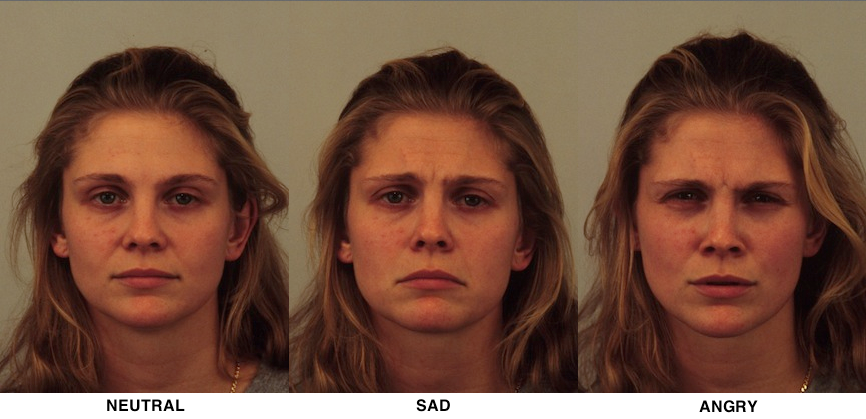
\includegraphics[scale=0.3]{figures/kdef_no_difference_emotions} 
=======
\noindent 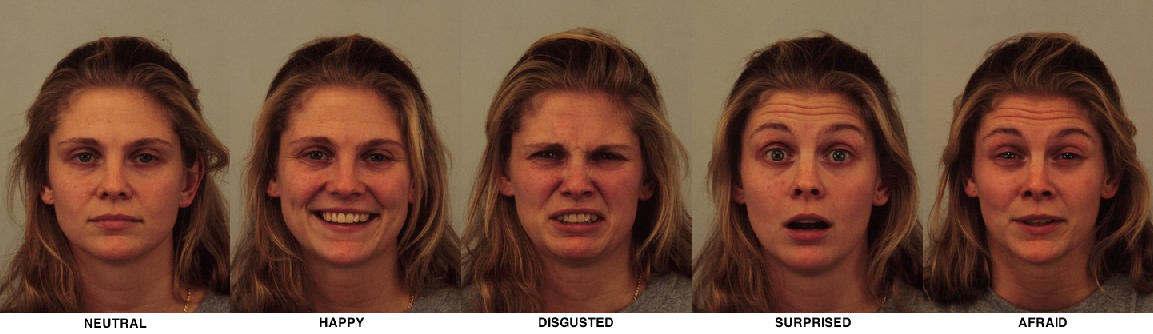
\includegraphics[scale=0.4]{figures/kdef_difference_emotions} 
>>>>>>> f3a1177041b834dbad80cc320be587f28fef16e6
\newline
\caption{Face images from the KDEF database used in the test set}
\label{kdef_difference_emotions}
\end{center} 
\end{figure}

\noindent As it can be seen in Figure~\ref{kdef_difference_emotions}, for each emotion, eyebrows are raised, eyes are widely opened, and the mouth has a distinct shape, whereas in Figure~\ref{kdef_no_difference_emotions} there are no differences as visible as in Figure~\ref{kdef_difference_emotions}. These variations of intensity might explain why the system struggles when trying to differentiate \textit{angry} and \textit{sad} emotional states.
\newline

\noindent The second group contains the 2 remaining facial expressions. The 2 facial expressions \textit{angry} and \textit{sad}, are the ones that distort the less the face. For a same subject expressing these 2 different emotions, as in Figure~\ref{kdef_no_difference_emotions}, the differences are not clearly noticeable.
\newline

\begin{figure}[!h]
\begin{center}
\noindent 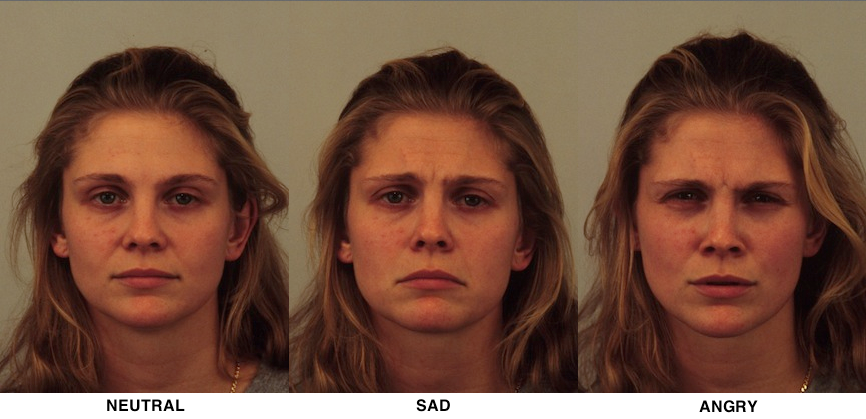
\includegraphics[scale=0.5]{figures/kdef_no_difference_emotions} 
\newline
\caption{Face images from the KDEF database used in the test set}
\label{kdef_no_difference_emotions}
\end{center} 
\end{figure}

\noindent The \textit{sad} emotion is the one that is the hardest to recognize. On 12 times, it has been well recognized only once. It is mostly taken for the \textit{neutral} state. As it can be seen in the Figure~\ref{kdef_no_difference_emotions}, there is not clear change between the \textit{neutral} state and the \textit{sad} emotion. Only the eyebrows are lightly frowned.
\newline

\noindent The \textit{angry} emotion is also hard to recognize. On 12 times, it has been well recognized only 5 times. It is mostly taken for the \textit{neutral} state and for the \textit{angry} emotion. As it can be seen in the Figure~\ref{kdef_no_difference_emotions}, there is not clear change between the \textit{neutral} state, the \textit{sad} emotion and the \textit{angry} emotion. Only the eyebrows slightly change as the eyes. The mouth is almost identical between the three face images in the Figure~\ref{kdef_no_difference_emotions}
\newline

\phantomsection
\section{Second result set}

\vspace{\baselineskip}
\noindent The second result test is processed in the same way as the first data set, the only difference being the input. Indeed, it is not performed on static images extracted from the KDEF database anymore; images used for texting are extracted from the video stream coming from the Kinect. A subject stands in front of the Kinect, his or her face is detected and extracted, then features are computed, and finally classification is performed. It runs almost in real-time, and the process outputs the name of the emotion expressed.
\newline

\subsection{With face images from the KDEF database}

\vspace{\baselineskip}
\noindent Because the results do not have a good accuracy at first sight, another method is tested. Face images from the KDEF database are printed on A4 paper and are put in front of the Kinect.
\newline

\noindent GIVE THE RESULTS OBTAINED
\newline

\subsection{With subjects}

\vspace{\baselineskip}
\noindent GIVE THE RESULTS OBTAINED
\newline

